\documentclass[10pt, a4paper]{article}
\usepackage[margin=0.75in]{geometry}
\usepackage{graphicx}
\usepackage{wrapfig}
\usepackage{caption}
\usepackage{subcaption}
\usepackage{hyperref}
\usepackage[table]{xcolor}% http://ctan.org/pkg/xcolor
\graphicspath{{images/}}

\title{Applied Machine Learning - Sentiment Analysis}
\author{Poppy Z Grimes, Pinar Batat Buke, Zhifan Sun}
\date{November 2022}


\begin{document}
\maketitle 

\section{Task description}

This project performs an exploratory sentiment analysis on film reviews in the Stanford Sentiment Treebank (SST-5) dataset with some supplementary datasets. We apply various supervised and unsupervised classification models to assess their performance in determining sentiment of online film reviews. We approach this by generating models for binary and multiclass classification. We explore the difference in performance when feeding models with input features from full sentences or phrases. The highest performing model is then optimised to enhance performance. 

 In addition, we demonstrate how pre-processing techniques effect our outcomes. This includes lemmetisation and human sentiment subjectivity. Ultimately, we investigate whether we can build accurate models for fine-grained sentiment from this data. %does it outperform binary?



\section{Background and related work}

%SST dataset, how files are split, previous wok on it 
%what is sentiment analysis 

The SST-5 dataset is a repository of 11855 film review sentences from RottenTomatoes.com. The repository is organised into several files which split the data into sentences or phrases. Phrases from reviews have human-assigned sentiment scores where participants were asked to score on a continuous sliding scale seen in figure \ref{fig:sentiment_scale}.

\begin{wrapfigure}{l}{0.3\textwidth}
    \begin{center}
        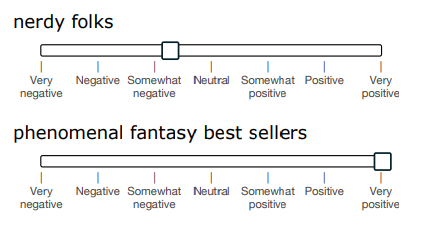
\includegraphics[width=0.189\textwidth]{sentiment_scale} 
    \end{center}
\caption{Continuous sentiment scale}
\label{fig:sentiment_scale}
\end{wrapfigure}

From this, phrases were assigned into one of five sentiment classes, producing a fine-grained sentiment labelled dataset. Unlike binary data, having five discrete classes overcomes the limitation of binary classifiers when faced with dual polarity (cite). A noteworthy example of this can be seen in negation \textit{e.g. 'this film hardly made me laugh'}. 

\subsection{Training on a recursive Neural Tensor Network (RNTN)}
This dataset was initially introduced by Socher \textit{et al.} (2013) to test a new neural network model with the aim to outperform previous algorithms on a) binary classification and b) fine-grained sentiment labels.

We also identified an analysis by Rao (2019) who took a similar approach to us in attempting to classify whole-sentences

\subsection{Bag of words (BOW)}
Bag of words is a popular method which tracks the polarity of individual words. It can be used to weight particularly positive or negative individual words accordingly. As a result, it is more successful in longer text strings. BOW exhibits weakness in that it does not account for grammatical, semantic or structural features within language. We decided to implement this as a baseline comparison but with the expectation of low performance.



\section{Task significance}

Sentiment analysis is one of the cornerstones of natural language processing (NLP) to classify the positive or negative feeling within human text or speech. In the context of machine learning algorithms, sentiment analysis can be performed using both supervised and unsupervised methods. 

Sentiment analysis is a popular tool used by businesses to gain insight into customer preferences, make suggestions based on consumer opinion and understand patterns and trends in social media. Fine-graining sentiment analysis is particularly challenging due to the nuances, rule exceptions and other linguistic features of the English - and in fact every - language. Understanding human behaviour and opinion is extremely valuable for those wanting to apply such data into marketing, social, political and other applications. Machine learning has wielded such endeavours with the tools to do so.

The diversity of machine learning techniques, and by their nature, means that we can arrive at almost the same outputs given various inputs and models. Therefore, determining the best performing model in terms of speed, accuracy and optimisation is the crux of most exploratory analyses. The rationale of this work is build on that notion where we are taking multiple approaches to the same question see how we can arrive optimally to our solutions. 



%can we choose best classifier to put in any new data point x and accurately assign it to a binary or multiclass feature label 





\section{Information on Data Pre-processing}

\subsection{Phrase pre-processing steps}

\begin{enumerate} 
    \item Align each phrase with its label using the phrase ID by combining dictionary.txt and sentiment\_labels.txt
    \item Classify labels into discrete bins from the range [0,1] into classes ranging from 1 to 5
    \item Lemmetisation
    \begin{enumerate}
        \item Using \textit{Stanza} library get lemma of each word in phrases returning either verb, adjective, adverb
        \item Also select for word "not" in each phrase (negation)
        \item Using \textit{NLTK} library remove stop words 
    \end{enumerate}
    \item Create a dataframe with columns: $['id', 'phrase', 'lemma', 'key\_words', 'label'],$ where $key\Uwords$ column contain the verbs, adjective and adverb of each phrase.
\end{enumerate}
    
    lemma provides highest value information
    
    %sentiment score is weighted from [0,1] put into binary or discrete classes by *5 probabiliy

\subsection{Sentence pre-processing}

\subsubsection{Assigning sentiment scores to sentences}
The provided data set assigns sentiment scores only to individual phrases, or n-grams. For the purpose of our supervised analysis, we need sentiment labels for full sentences. The first method we have chosen is to manually score (human-based) a random sample of n=100 sentences as positive or negative. This will be a test dataset.

A second method we explore is using the x function in NLTK library which generates a portfolio of scores for each datapoint for positive, neutral and negative. From this we compute a compound score in the range [0,1]. 

%sentences not lablled: two methods human and external NLTK package with compound score and perform supervised classification on compound score




Second, we have pulled positive and negative words with high polarity with assigned sentiment from the labelled phrase-bank. For both routes, these will act as labels for training our classifiers. 










\section{Exploratory data analysis}

\subsection{Phrase Analysis}
\subsubsection{Word Clouds}
We drew word cloud images for each class, and for both the lemma data and the key\_word data. Keywords appear to be more relevant with the label Figures \ref{fig:classcloud} and \ref{fig:lemmacloud}.

\begin{figure}[h]
     \centering
     \begin{subfigure}[b]{0.18\textwidth}
         \centering
         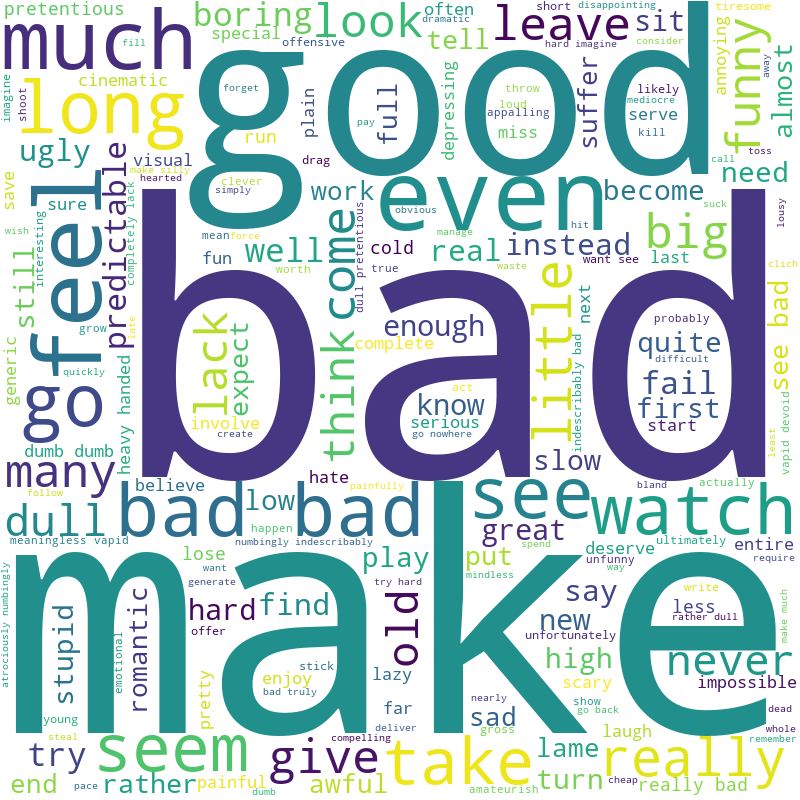
\includegraphics[width=\textwidth]{keywords1.png}
         \caption{Class 1}
         \label{fig:class1cloud}
     \end{subfigure}
     \hfill
     \begin{subfigure}[b]{0.18\textwidth}
         \centering
         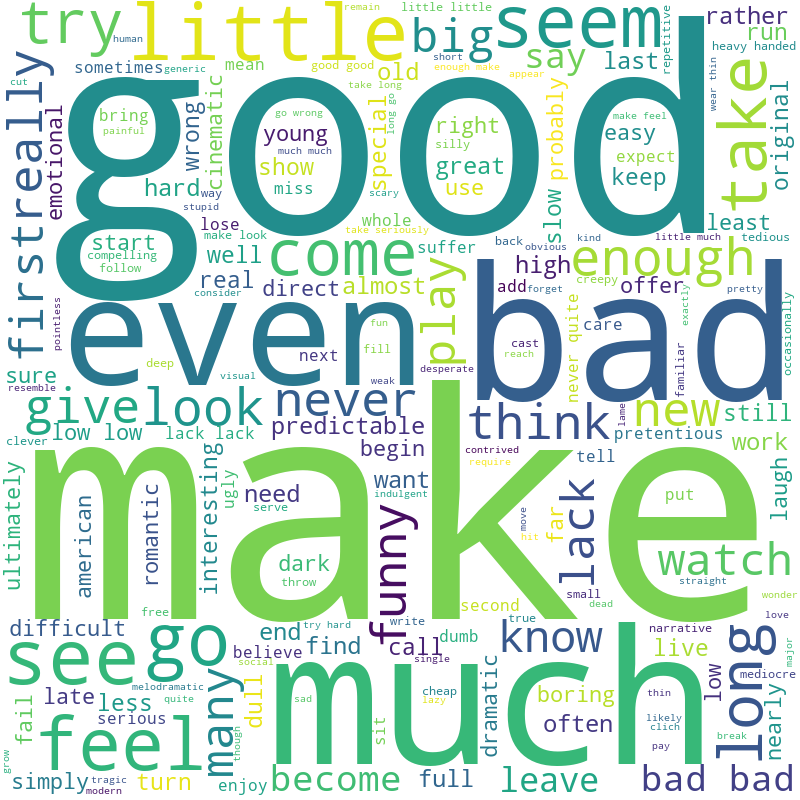
\includegraphics[width=\textwidth]{keywords2.png}
         \caption{Class 2}
         \label{fig:class2cloud}
     \end{subfigure}
     \hfill
     \begin{subfigure}[b]{0.18\textwidth}
         \centering
         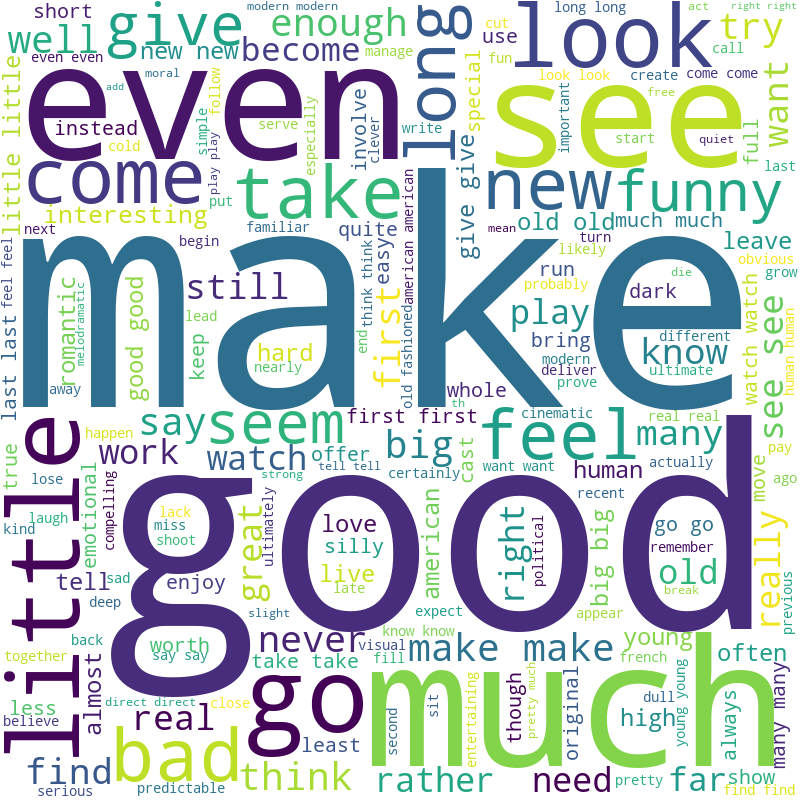
\includegraphics[width=\textwidth]{keywords3.png}
         \caption{Class 3}
         \label{fig:class3cloud}
     \end{subfigure}
     \hfill
     \begin{subfigure}[b]{0.18\textwidth}
         \centering
         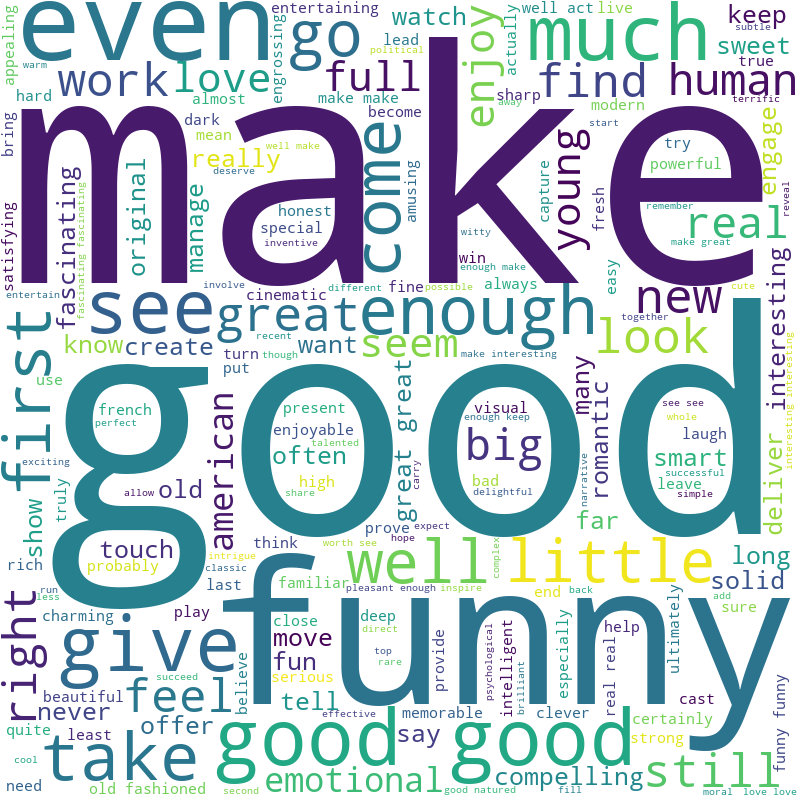
\includegraphics[width=\textwidth]{keywords4.png}
         \caption{Class 4}
         \label{fig:class4cloud}
     \end{subfigure}
     \hfill
     \begin{subfigure}[b]{0.18\textwidth}
         \centering
         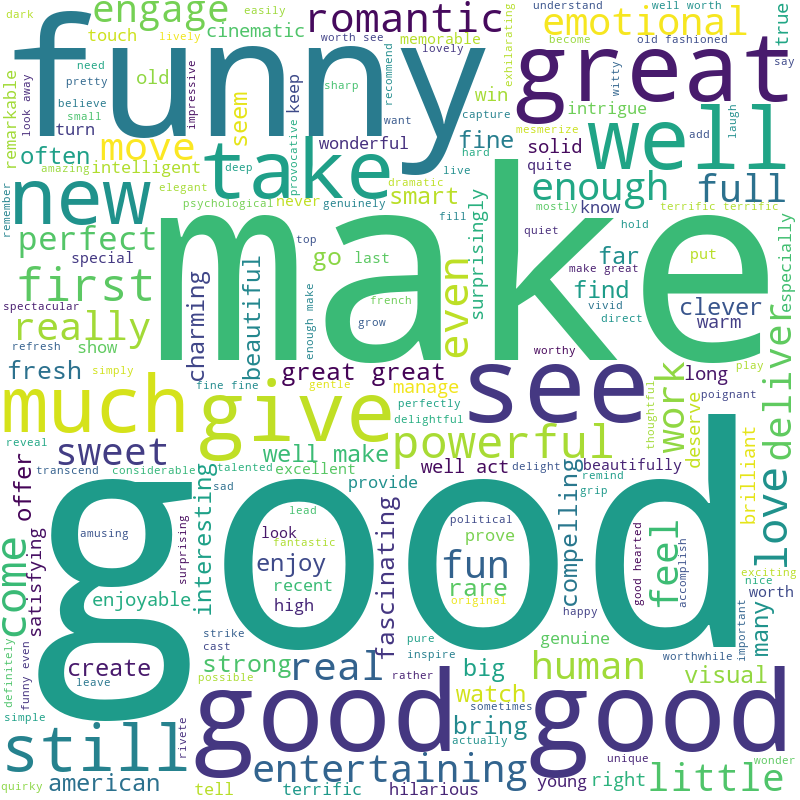
\includegraphics[width=\textwidth]{keywords5.png}
         \caption{Class 5}
         \label{fig:class5cloud}
     \end{subfigure}
     \hfill
    \caption{Word clouds for keywords in each class}
\label{fig:classcloud}
\end{figure}
\begin{figure}[h]
     \centering
     \begin{subfigure}[b]{0.18\textwidth}
         \centering
         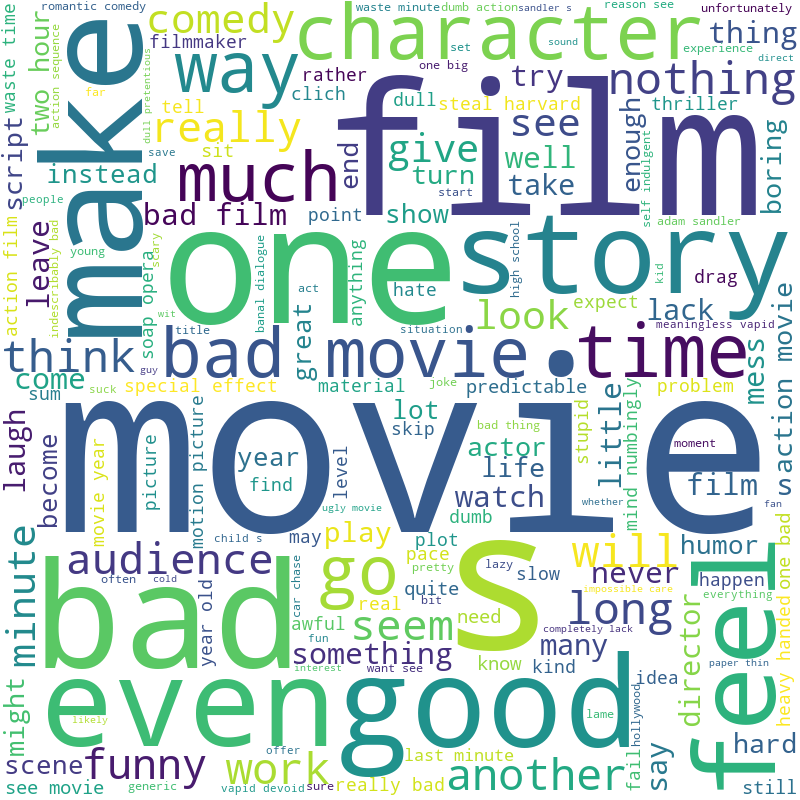
\includegraphics[width=\textwidth]{lemma1.png}
         \caption{Class 1}
         \label{fig:lemma1cloud}
     \end{subfigure}
     \hfill
     \begin{subfigure}[b]{0.18\textwidth}
         \centering
         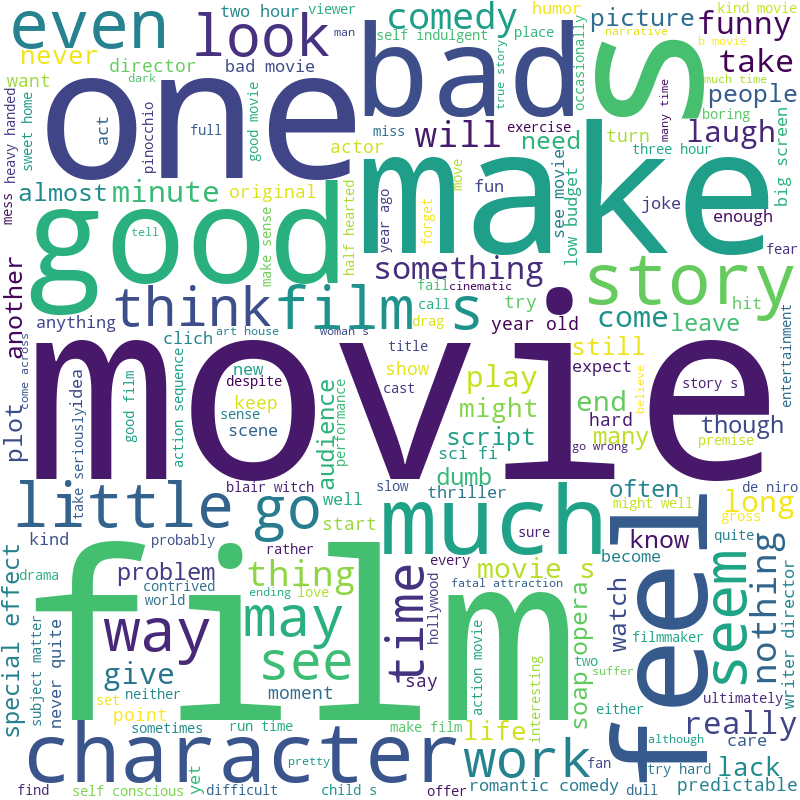
\includegraphics[width=\textwidth]{lemma2.png}
         \caption{Class 2}
         \label{fig:lemma2cloud}
     \end{subfigure}
     \hfill
     \begin{subfigure}[b]{0.18\textwidth}
         \centering
         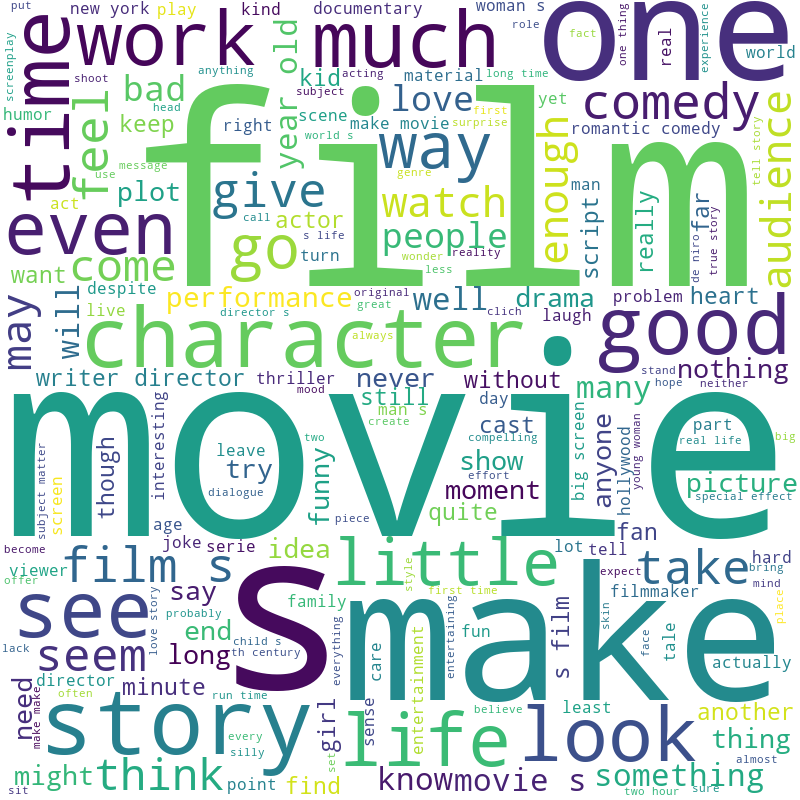
\includegraphics[width=\textwidth]{lemma3.png}
         \caption{Class 3}
         \label{fig:lemma3cloud}
     \end{subfigure}
     \hfill
     \begin{subfigure}[b]{0.18\textwidth}
         \centering
         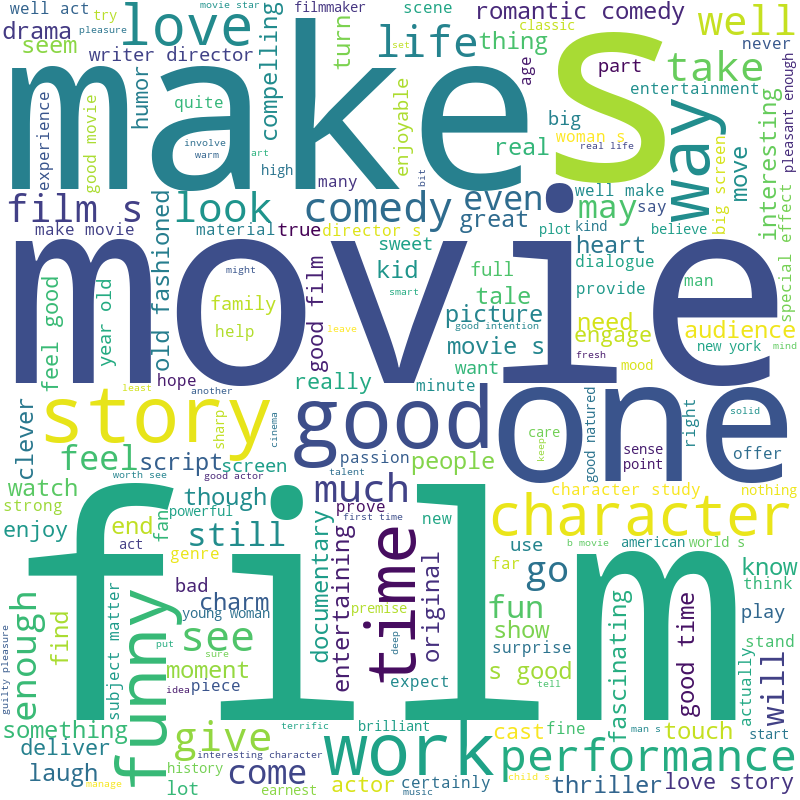
\includegraphics[width=\textwidth]{lemma4.png}
         \caption{Class 4}
         \label{fig:lemma4cloud}
     \end{subfigure}
     \hfill
     \begin{subfigure}[b]{0.18\textwidth}
         \centering
         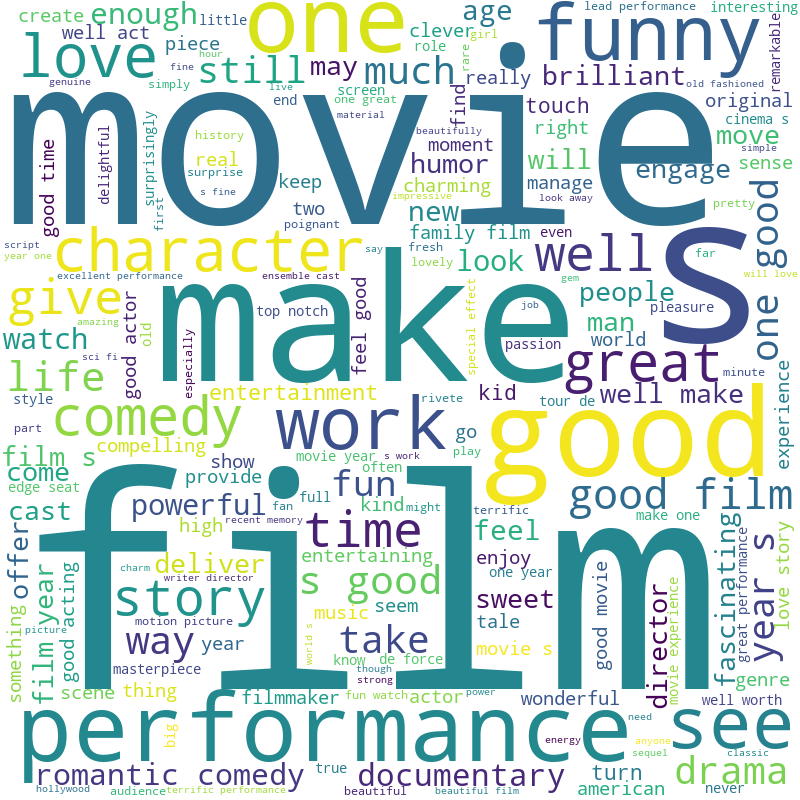
\includegraphics[width=\textwidth]{lemma5.png}
         \caption{Class 5}
         \label{fig:lemma5cloud}
     \end{subfigure}
     \hfill
    \caption{Word clouds for lemma in each class}
\label{fig:lemmacloud}
\end{figure}

To choose our input features we selected the 16 most frequent words from each class and additionally hand-picked 15 from the word-clouds. This brought us to a total of 95 keyword features. We performed supervised classification using three classes (positive, neutral and negative).


\subsection{Sentence Analysis}
We use an \href{http://ai.stanford.edu/~amaas/data/sentiment/}{external dataset} \cite{maas2011learning} to train our model for the sentence-based analysis as sentences are unlabelled in the SST-5 and we only had capacity on this occasion to hand-label 100. Our training dataset is from the IMDB movie review platform with n = 25,000 datapoints (sentences) labelled as positive or negative, following the same structure and inputs of our test data. We initially split the IMDB data into test (80\%) and train (20\%) before testing with our human-labelled the SST-5 data.





\section{Description of learning methods used}

\subsection{Supervised models}
\begin{itemize}
    \item \textbf{Naive Bayes (NB)} - A generative linear classifier built on Bayes' theorem which predicts the probability of class label $Y$ given input features $X$. This is indirectly computed through the likelihood $P(X|Y)$ and prior $P(Y)$. Assumption: Features are independent and identically distributed (IID) given the class. Advantage: Fast and powerful on smaller datasets.
    
    \item \textbf{Logistic Regression (LR)} - [binary] A discriminative linear classifier that directly computes $P(Y|X)$ using weighted input features $w_{i}x_{i}$ and the sigmoid function $σ(z) = 1/(1+e^-^z))$ where $z$ is the sum of weighted features plus the bias term (scalar intercept). Data is normalised between [0,1] and a decision boundary (classification threshold, usually 0.5) predicts $P(Y|X)$. Advantage: Splits weights between input features that correlate, therefore doesn't assume independence. \\
    
    [multinomial] For multiple classes, multinomial LR uses one-hot vectors as the output $Y$. The classifier predicts $\hat{y}$ given $x_{i}$ from probabilities of one-hot vectors.
    
    \item \textbf{Decision Tree (DT} - A non-linear method which iteratively partitions inputs starting with a 'root' node. Inputs descend through top-down questions that split data based on attributes of input features, returning class probabilities at the terminating leaf nodes. Thresholds of each branch are established by measuring node entropy, where the aim is to minimise entropy to have high purity (data points from same class at same node). Advantage: Fast and clear classification with specified set of input features.
    
    \item \textbf{Random Forest (RF)} - An ensemble of $k$ DT's where subsets of data and random feature subsets are split and trained across the various trees. The learning is repeated $k$ times (cross-validation?). Classes of datapoints are predicted from a 'majority vote' across all of the trees. Advantage: Powerful on big data. Pitfall: Longer time, lower interpretability.
\end{itemize}\\\



\section{Results and evaluation}
\subsection{Performance on sentences}

\begin{wraptable}{r}{80mm}
\parbox{.45\linewidth}{
\centering
\begin{tabular}{||c c c c||} 
 \hline
 Classifier & Accuracy & F1 score &\\ [0.5ex] 
 \hline\hline
 Naive Bayes' & 0.406 & 0.285 &\\ 
 \hline 
 Logistic Regression & \cellcolor{yellow!25}0.723 & 0.724 &\\
 \hline
 Decision Tree & 0.634 & 0.578 &\\
 \hline
 Random Forest & 0.644 & 0.577  &\\
 \hline\hline
\end{tabular}
\caption{Human-based}
\label{table:human}
}

\parbox{0.45\linewidth}{
\centering
\begin{tabular}{||c c c c||} 
 \hline
 Classifier & Accuracy & F1 score &\\ [0.5ex] 
 \hline\hline
 Naive Bayes' & 0.733 & 0.723 &\\ 
 \hline 
 Logistic Regression & \cellcolor{yellow!25}0.876 & 0.876 &\\
 \hline
 Decision Tree & 0.718 & 0.717 &\\
 \hline
 Random Forest & 0.847 & 0.846  &\\
 \hline\hline
\end{tabular}
\caption{NLTK library}
\label{table:nltk}
}
\end{wraptable}

Results in Table \ref{table:human} and Table \ref{table:nltk} were performed on training data from the IMDB dataset. LR showed highest performance for classifying whole sentence sentiment for both our human-labelled test data (SST-5) and IMDB test data, highlighted in yellow. Sentiment data for words likely includes correlated input features, especially with the combination of adverbs and adjectives which strengthen polarity of sentiment. Poor performance of NB on our human-labelled sentences perhaps reflects the model's IID assumption.






\subsubsection{Using NLTK compound scores}


\section{Conclusions}



\bibliographystyle{plain}
\bibliography{bibliography}

\end{document}